\documentclass[prd,aps,amsfonts,amsmath, nofootinbib]{revtex4}
\input{epsf}
\usepackage{graphicx}
\usepackage{thumbpdf}
\usepackage{pdfsync}
%\usepackage[pdftex]{graphicx}


\def\be{\begin{equation}}
\def\en{\end{equation}}
\def\bea{\begin{eqnarray}}
\def\ena{\end{eqnarray}}

\begin{document}
\title{Preliminary evaluation of MLDC SMBH challenge: Round 1}
\author{S. Babak, E. Porter, M. Vallisneri}
\maketitle

\section{Challenge evaluation}

Three collaborations have submitted results for the challenge 1.2.1. Two submissions contain estimation of all nine parameters and the third 
one contains estimation of only chirp mass and time of coalescence.
We have only one entry for challenge 1.2.2.

In order to evaluate the results we have computed several quantities.
The noise weighted inner products were computed using $X$-stream
(used in MLDC) and two orthogonal streams with equal and uncorrelated 
noise:

\bea
A = (2X - Y - Z)/3; \;\;\;\; E = (Z - Y)/\sqrt{3}
\ena
and approximate expression for the noise \bea
S = 2(S_X - S_{XY})/3
\ena
where for the frequency response used in synthetic LISA:
\bea
S_X &=& 16 \sin^2(2\pi fL)  (2 (1 + \cos^2(2\pi fL)) S_{pm} + S_{op})\\
S_{XY} &=& -4 \sin(4\pi fL)\sin(2\pi fL)  ( S_{op} + 4S_{pm} )\\
S_{pm} &=& 2.5\times10^{-48} \left(1 + \left(\frac{f}{10^{-4}Hz}\right)^{-2}
\right)  \left(\frac{f}{1Hz}\right)^{-2},\;\;\;
S_{op} = 1.8\times 10^{-37}  \left(\frac{f}{1Hz}\right)^2
\ena
We have computed the following quantities. The $\xi^2$ per degree
of freedom
\bea
\chi^{2} = \frac{(A_{data}- A_{rec}|A_{data}- A_{rec}) + 
(E_{data} - E_{rec}|E_{data} - E_{rec})}
{N-D}
\ena
and another (similar) quantity

\bea
\xi = \frac{\sqrt{(A_{data}- A_{rec}|A_{data}- A_{rec})^2 + 
(E_{data} - E_{rec}|E_{data} - E_{rec})^2}}
{N-D}
\ena
where $N$ is a number of points and $D=9$ is number of parameters.

The second value is recovered combined SNR:
\bea
SNR = \sqrt{SNR_A^2 + SNR_E^2},\\
SNR_A = \frac{(A_{data}|A_{rec})}{\sqrt{(A_{rec}|A_{rec})}},\;\;\;
SNR_E = \frac{(E_{data}|E_{rec})}{\sqrt{(E_{rec}|E_{rec})}}
\ena
Together with this we also compare noiseless injected signal with 
the recovered one. Here we compute several overlaps:
\bea
O_A = \frac{(A_{key}|A_{rec})}{\sqrt{(A_{rec}|A_{rec})(A_{key}|A_{key})}}, \;\; 
O_E = \frac{(E_{key}|E_{rec})}{\sqrt{(E_{rec}|E_{rec})(E_{key}|E_{key})}}
\ena
and overlap of difference between $X$ channels:
\be
O_{dX} = \frac{(X_{rec}-X_{key}|X_{rec}-X_{key})}
{\sqrt{(X_{rec}|X_{rec})(X_{key}|X_{key})}}
\en
Overlaps show how well we track the phase neglecting error in 
the amplitude.

In order to take into account the possible error in the initial 
phase we have computed overlaps maximized over the phase:

\bea
max_{\phi_0}(O_X) = \sqrt{(X_{rec}|X_{key}(\phi_0 = 0))^2 +
(X_{rec}|X_{key}(\phi_0 = \pi/2))^2}\\
min_{\phi_0}(O_{dX}) = \frac{ (X_{rec}|X_{rec}) + (X_{key}|X_{key}) -
2 max_{\phi_0}(X_{rec}|X_{key})}{\sqrt{(X_{rec}|X_{rec})(X_{key}|X_{key})}}
\ena

We have also computed errors in the parameter estimations in units 
of sigma. Sigma was taken from the diagonal elements of (inverse of) Fisher matrix. Numerical values of Fisher matrix were checked against
LISA calculator.

Finally we plot noiseless data and provide visual comparison of the 
recovered signals against the key.

\section{Challenge1.2.1}

We denote three entries as Montana/AEI, JPL, Goddard.
Results of computing various inner products are summarized in the 
Table~\ref{OlapsTable1.2.1}. Montana/AEI entry have constant phase difference (which is clear from values of
maximized overlaps), we have added one more entry (Montana/AEI*) with corrected initial phase.

\begin{table}
\caption{\label{OlapsTable1.2.1} Inner products for challenge 1.2.1}
\begin{ruledtabular}
\begin{tabular}{|c|c|c|c|c|c|c|c|c|}
Entry & $\chi^2$ & $\xi$ & SNR & $O_A$ & $O_E$ & $O_{dX}$ & $min_{\phi_0}(O_{dX})$ & $max_{\phi_0}(O_X)$\\
\hline
Key & 0.5824 & 0.41182 & 667.734 &  -- & -- & -- & -- & -- \\
Montana/AEI & 0.67193 & 0.47606 & 528.023 & 0.79153 & 0.79051 &
0.41694 & 0.000128 & 0.99994\\
JPL & 0.58451 & 0.41331 & 664.471 & 0.9944 & 0.9958 & 0.0112 &  0.00909 & 0.9955\\
Montana/AEI* & 0.58331 & 0.412466 & 666.324 & 0.998 & 0.998 & 0.0112 & 0.000128 & 0.99994 \\
\hline
\end{tabular}
\end{ruledtabular}
\end{table}

%The 9-d covariance matrix represented by $\ln(Mc), \ln(mu), \ln(DL), colatitude, phi, inclination, psi, \ln(tc), phi_c$
%\be
%\left( \begin{array}{ccccccccc}
 %3.872372e-10  &   5.487736e-09 &   -4.830902e-08 &  -6.512430e-09 &  3.874956e-09  &  -2.797328e-08  & -1.947460e-08   & 6.921398e-12  &  6.832675e-07\\
 %5.487736e-09   &  8.895662e-08  &  -4.304437e-07  &  1.219430e-08 & -6.682858e-08  &  -7.488979e-08  &  3.690754e-07   1.161215e-10   & 1.401720e-05\\
%-4.830902e-08  &  -4.304437e-07   &  3.040359e-04 &   1.676021e-05 &  7.627013e-06  &   1.280722e-04 &  -1.853579e-05  -6.568543e-12  & -1.714562e-05\\
%-6.512430e-09  &   1.219430e-08  &   1.676021e-05  &  3.293878e-06 & -2.384544e-06  &   1.123548e-05  &  1.171880e-05  -1.322383e-11  &  4.981729e-05\\
% 3.874956e-09  &  -6.682858e-08  &   7.627013e-06  & -2.384544e-06 &  4.513706e-06  &  -2.712281e-06 &  -1.819819e-05   2.635738e-11   &-7.240383e-05\\
%-2.797328e-08  &  -7.488979e-08  &   1.280722e-04  &  1.123548e-05 & -2.712281e-06  &   6.417406e-05  &  2.222767e-05   %7.460451e-12   & 1.138302e-04\\
%-1.947460e-08  &   3.690754e-07  &  -1.853579e-05  &  1.171880e-05 & -1.819819e-05  &   2.222767e-05  &  9.518923e-05   5.743921e-11   & 3.779646e-04\\
% 6.921398e-12  &   1.161215e-10  &  -6.568543e-12  & -1.322383e-11 &  2.635738e-11  &   7.460451e-12 &   5.743921e-11   1.707089e-13   & 1.785465e-08\\
% 6.832675e-07  &   1.401720e-05  &  -1.714562e-05  &  4.981729e-05 & -7.240383e-05  &   1.138302e-04  &  3.779646e-04   1.785465e-08   & 3.398534e-03

% 3.87e-10  &   5.49e-09 &   -4.83e-08 &  -6.51e-09 &  3.87e-09  &  -2.8e-08  & -1.95e-08   & 6.92e-12  &  6.84e-07\\
% 5.49e-09   &  8.9e-08  &  -4.30e-07  &  1.22e-08 & -6.68e-08  &  -7.49e-08  &  3.69e-07 &  1.16e-10   & 1.40e-05\\
%-4.83e-08  &  -4.30e-07   &  3.04e-04 &   1.68e-05 &  7.63e-06  &   1.28e-04 &  -1.85e-05 & -6.57e-12  & -1.71e-05\\
%-6.51e-09  &   1.22e-08  &   1.68e-05  &  3.29e-06 & -2.38e-06  &   1.12e-05  &  1.17e-05 & -1.32e-11  &  4.98e-05\\
% 3.87e-09  &  -6.68e-08  &   7.63e-06  & -2.38e-06 &  4.51e-06  &  -2.71e-06 &  -1.82e-05 &  2.63e-11   &-7.24e-05\\
%-2.8e-08  &  -7.49e-08  &   1.28e-04  &  1.12e-05 & -2.71e-06  &   6.42e-05  &  2.22e-05  & 7.46e-12   & 1.14e-04\\
%-1.95e-08  &   3.69e-07  &  -1.85e-05  &  1.17e-05 & -1.82e-05  &   2.22e-05  &  9.52e-05 &  5.74e-11   & 3.78e-04\\
% 6.92e-12  &   1.16e-10  &  -6.57e-12  & -1.32e-11 &  2.63e-11  &   7.46e-12 &   5.74e-11 &  1.71e-13   & 1.79e-08\\
% 6.83e-07  &   1.40e-05  &  -1.71e-05  &  4.98e-05 & -7.24e-05  &   1.14e-04  &  3.78e-04 &  1.79e-08   & 3.4e-03
%\end{array}
%\right)
%\en
%Note that off diagonal elements represented by correlation with actual parameters, not $\ln$ ({\bf Ed please confirm it}).
%This corresponds to the following values of one sigma deviation for a given in challenge 1.2.1 parameter set:
The variance-covariance matrix provides us with the following values for sigma

\bea
M_c = 1.208590\times 10^6,\;\;\;     \sigma = 23.78306\\
\mu = 5.811961\times 10^5,\;\;\;     \sigma = 173.3452\\
Dl = 8.000000,\;\;\;     \sigma = 0.1394930\\
colat = -0.492289, \;\;\;   \sigma = 0.0018149\\
long = 0.865777 , \;\;\;      \sigma = 0.00212455\\
inc = 1.94439 , \;\;\;       \sigma = 0.00801087\\
\psi = 3.23422, \;\;\;        \sigma = 0.0097565\\
t_c = 1.337403\times 10^7,\;\;    \sigma = 5.525738\\
\phi_c = 4.364670, \;\;\;      \sigma = 0.058297
\ena

{\bf Ed, I have noticed that colatitude here is actually latitude!}

The errors in the parameter estimation (in units of sigma) are presented in the Table~\ref{Errors1.2.1}
\begin{table}
\caption{\label{Errors1.2.1} Errors in estimation of parameters for challenge 1.2.1. Values in brackets corresponds to the 
opposite direction on the sky.}
\begin{ruledtabular}
\begin{tabular}{|c|c|c|c|c|c|c|c|c|c|}
Entry & $\Delta M_c$ & $\Delta \mu $ & $\Delta Dl$ & $\Delta \theta $ & $\Delta \phi $ & $\Delta inc $ &
$\Delta \psi $ & $\Delta t_c $& $\Delta \phi_c $ \\ 
\hline
 JPL & 37.3& 36.8 &-63.2 & 566.308 (23.75)& -1493.76  (-15.08) & 165.719 & -271.752 & -8.1 &
0.074\\
Montana/AEI & -5.0 & -3.5 & 2.4  & 0.63 & 0.63 & 2.1 & 322.0 & -0.62 &  0.076 \\
Goddard & -2203 & -- & --  & --& -- & -- & -- & -- & -1433 \\
\hline
\end{tabular}
\end{ruledtabular}
\end{table}


Finally in the Figure~\ref{fig1.2.1} we compare beginning and the end of the recovered signals as compared
to key. 
\begin{figure}[ht]
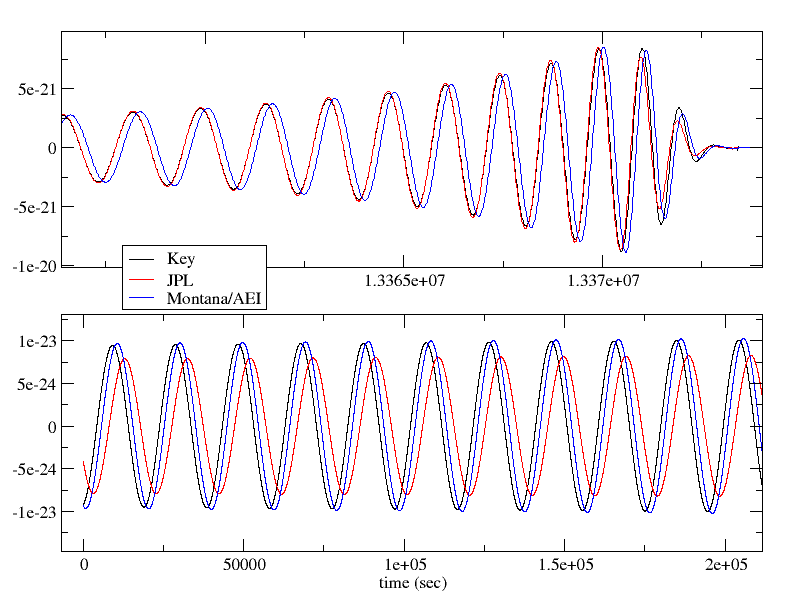
\includegraphics[height=0.6\textheight,
keepaspectratio=true,angle=0]{1_2_1X}
\caption{Comparison of the $X$-response to the signal from inspiralling SMBH. }
\label{fig1.2.1}
\end{figure}

JPL signal provides a very good fit to the key in the LISA's most sensitive frequency band, but not across 
the whole bandwidth.

 
\section{Challenge1.2.2}

There is only one entry for this challenge. Here we present only inner product results, which are summarized in the
Table~\ref{OlapsTable1.2.2}

\begin{table}
\caption{\label{OlapsTable1.2.2} Inner products for challenge 1.2.2}
\begin{ruledtabular}
\begin{tabular}{|c|c|c|c|c|c|c|c|c|}
Entry & $\chi^2$ & $\xi$ & SNR & $O_A$ & $O_E$ & $O_{dX}$ & $min_{\phi_0}(O_{dX})$ & $max_{\phi_0}(O_X)$\\
\hline
Key & 0.58063 & 0.410566 & 106.77 & -- & -- & -- & -- & -- \\
Montana/AEI & 0.58064 & 0.41058 &  106.60 & 0.9984 & 0.9987 & 0.0033 & 0.0029 & 0.9985 \\
\hline
\end{tabular}
\end{ruledtabular}
\end{table}

And visual comparison (again beginning and the end) is presented in the figure~\ref{fig1.2.2}.

\begin{figure}[ht]
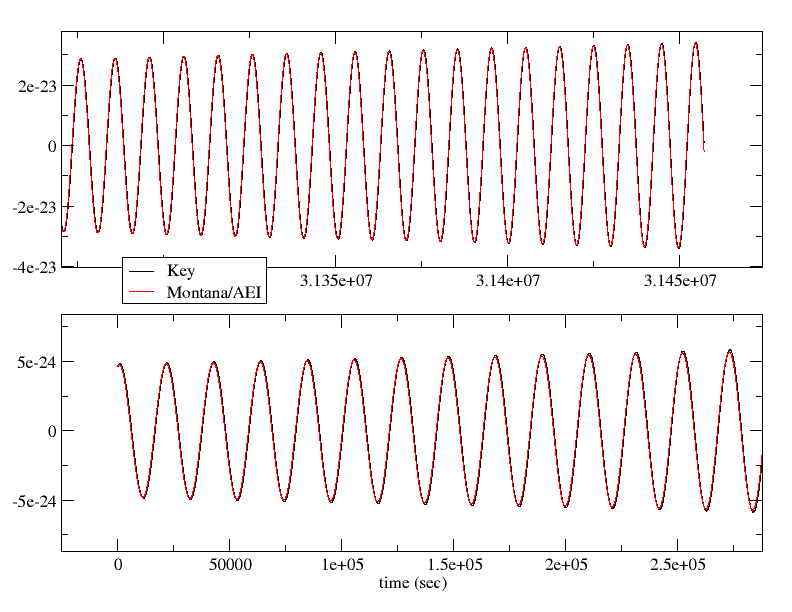
\includegraphics[height=0.6\textheight,
keepaspectratio=true,angle=0]{Eval122.png}
\caption{Comparison of the $X$-response to the signal from inspiralling SMBH. }
\label{fig1.2.2}
\end{figure}

\end{document}
